%%===========================================================%%
%%                                                           %%
%%                     RpEfficiencySystematicsAppendix                  %%
%%                                                           %%
%%===========================================================%%

\chapter{RP track reconstruction efficiency comparison between data and MC}\label{appendix:rpTrackRecoEffSyst}\vspace{-26pt}


%---------------------------
\begin{figure}[h]%\vspace{-34pt} 
	\centering
	\parbox{0.54\textwidth}{
		\centering
		\begin{subfigure}[b]{\linewidth}{\vspace{10pt}
				\subcaptionbox{\label{fig:totalRpRecoEff2D_ED}}{\includegraphics[width=\linewidth,page=2]{graphics/systematicsEfficiency/RpSyst/totalRpRecoEff2D.pdf}\vspace{-12pt}}}
		\end{subfigure}
		\begin{minipage}[t][0.64\linewidth][t]{\linewidth}\vspace{10pt}
		\caption[Coparison of estimated RP track reconstruction efficiency in 2D and 1D (branch ED).]%
		{Comparison of RP track reconstruction efficiency in branch ED estimated with the method described in Sec.~\ref{subsec:rpTrackRecoEffSyst} as a function of $(p_{x},p_{y})$ of proton track (\ref{fig:totalRpRecoEff2D_ED}) and comparison of 1-dimensional projections of efficiencies in a fiducial region marked with green envelope: $p_{x}$ (\ref{fig:totalRpRecoEff1D_ED_px}) and $p_{y}$ (\ref{fig:totalRpRecoEff1D_ED_py}). Lower pad in each subfigure shows the difference between efficiency extracted from the data and elastic scattering MC embedded into zero-bias data. Hatched orange area marks bins without any entries (efficiency incalculable).}\label{fig:totalRpRecoEff_ED}
		\end{minipage}
		%\vspace{52pt}%
	}
	\quad
	\parbox{0.43\textwidth}{
		\centering
		\begin{subfigure}[b]{\linewidth}{
				\subcaptionbox{\label{fig:totalRpRecoEff1D_ED_px}}{\includegraphics[width=\linewidth,page=3]{graphics/systematicsEfficiency/RpSyst/dataTotalEff_1D.pdf}\vspace{-12pt}}}
		\end{subfigure}
		\begin{subfigure}[b]{\linewidth}{
				\subcaptionbox{\label{fig:totalRpRecoEff1D_ED_py}}{\includegraphics[width=\linewidth,page=4]{graphics/systematicsEfficiency/RpSyst/dataTotalEff_1D.pdf}\vspace{-12pt}}}
		\end{subfigure}
	}
\end{figure}
%---------------------------

%---------------------------
\begin{figure}\vspace{-154pt} 
	\centering
	\parbox{0.4725\textwidth}{%
		\centering%
		\includegraphics[width=\linewidth,page=2]{graphics/systematicsEfficiency/RpSyst/xiPerBranch.pdf}%
	} 
	\quad
	\parbox{0.4725\textwidth}{ 
		\centering\vspace{67pt}
		%\begin{minipage}[t][0.64\linewidth][t]{\linewidth}%\vspace{73pt} 
			\caption[Fractional momentum loss $\xi$ of clean proton tracks before and after implying vetoes in the data and MC (branch ED).]%
			{Fractional momentum loss $\xi$ of clean proton tracks in branch ED before and after implying vetoes. Data are represented by opened and filled circles, while elastic MC embedded into zero-bias data is drawn as filled histograms. MC histograms are scaled by the ratio of data and MC yields after imposing vetoes in other STAR detector subsystems. Lower pad shows the ratio of corresponding distributions in the data and MC. Dashed green vertical lines show the $\xi$ range of tracks accepted for the RP track (and also track point) efficiency studies, $|\xi|<0.01$.}\label{fig:rpSystXi_ED}%  
		%\end{minipage}
	}
	
\end{figure}
%---------------------------


%---------------------------
\begin{figure}[h]%\vspace{-34pt}
	\centering
	\parbox{0.54\textwidth}{
		\centering
		\begin{subfigure}[b]{\linewidth}{\vspace{10pt}
				\subcaptionbox{\label{fig:totalRpRecoEff2D_WU}}{\includegraphics[width=\linewidth,page=3]{graphics/systematicsEfficiency/RpSyst/totalRpRecoEff2D.pdf}\vspace{-12pt}}}
		\end{subfigure}
		\begin{minipage}[t][0.64\linewidth][t]{\linewidth}\vspace{10pt}
		\caption[Coparison of estimated RP track reconstruction efficiency in 2D and 1D (branch WU).]%
		{Comparison of RP track reconstruction efficiency in branch WU estimated with the method described in Sec.~\ref{subsec:rpTrackRecoEffSyst} as a function of $(p_{x},p_{y})$ of proton track (\ref{fig:totalRpRecoEff2D_WU}) and comparison of 1-dimensional projections of efficiencies in a fiducial region marked with green envelope: $p_{x}$ (\ref{fig:totalRpRecoEff1D_WU_px}) and $p_{y}$ (\ref{fig:totalRpRecoEff1D_WU_py}). Lower pad in each subfigure shows the difference between efficiency extracted from the data and elastic scattering MC embedded into zero-bias data. Hatched orange area marks bins without any entries (efficiency incalculable).}\label{fig:totalRpRecoEff_WU}
		\end{minipage}
		%\vspace{52pt}%
	}
	\quad
	\parbox{0.43\textwidth}{
		\centering
		\begin{subfigure}[b]{\linewidth}{
				\subcaptionbox{\label{fig:totalRpRecoEff1D_WU_px}}{\includegraphics[width=\linewidth,page=5]{graphics/systematicsEfficiency/RpSyst/dataTotalEff_1D.pdf}\vspace{-12pt}}}
		\end{subfigure}
		\begin{subfigure}[b]{\linewidth}{
				\subcaptionbox{\label{fig:totalRpRecoEff1D_WU_py}}{\includegraphics[width=\linewidth,page=6]{graphics/systematicsEfficiency/RpSyst/dataTotalEff_1D.pdf}\vspace{-12pt}}}
		\end{subfigure}
	}
\end{figure}
%---------------------------

%---------------------------
\begin{figure}%\vspace{-154pt} 
	\centering
	\parbox{0.4725\textwidth}{%
		\centering%
		\includegraphics[width=\linewidth,page=3]{graphics/systematicsEfficiency/RpSyst/xiPerBranch.pdf}%
	} 
	\quad
	\parbox{0.4725\textwidth}{ 
		\centering\vspace{67pt}
		%\begin{minipage}[t][0.64\linewidth][t]{\linewidth}%\vspace{73pt} 
			\caption[Fractional momentum loss $\xi$ of clean proton tracks before and after implying vetoes in the data and MC (branch WU).]%
			{Fractional momentum loss $\xi$ of clean proton tracks in branch WU before and after implying vetoes. Data are represented by opened and filled circles, while elastic MC embedded into zero-bias data is drawn as filled histograms. MC histograms are scaled by the ratio of data and MC yields after imposing vetoes in other STAR detector subsystems. Lower pad shows the ratio of corresponding distributions in the data and MC. Dashed green vertical lines show the $\xi$ range of tracks accepted for the RP track (and also track point) efficiency studies, $|\xi|<0.01$.}\label{fig:rpSystXi_WU}%  
		%\end{minipage}
	}
	
\end{figure}
%---------------------------




%---------------------------
\begin{figure}[h]%\vspace{-100pt}
	\centering
	\parbox{0.54\textwidth}{
		\centering
		\begin{subfigure}[b]{\linewidth}{\vspace{10pt}
				\subcaptionbox{\label{fig:totalRpRecoEff2D_WD}}{\includegraphics[width=\linewidth,page=4]{graphics/systematicsEfficiency/RpSyst/totalRpRecoEff2D.pdf}\vspace{-12pt}}}
		\end{subfigure}
		\begin{minipage}[t][0.64\linewidth][t]{\linewidth}\vspace{10pt}
		\caption[Coparison of estimated RP track reconstruction efficiency in 2D and 1D (branch WD).]%
		{Comparison of RP track reconstruction efficiency in branch WD estimated with the method described in Sec.~\ref{subsec:rpTrackRecoEffSyst} as a function of $(p_{x},p_{y})$ of proton track (\ref{fig:totalRpRecoEff2D_WD}) and comparison of 1-dimensional projections of efficiencies in a fiducial region marked with green envelope: $p_{x}$ (\ref{fig:totalRpRecoEff1D_WD_px}) and $p_{y}$ (\ref{fig:totalRpRecoEff1D_WD_py}). Lower pad in each subfigure shows the difference between efficiency extracted from the data and elastic scattering MC embedded into zero-bias data. Hatched orange area marks bins without any entries (efficiency incalculable).}\label{fig:totalRpRecoEff_WD}
		\end{minipage}
		%\vspace{52pt}%
	}
	\quad
	\parbox{0.43\textwidth}{
		\centering
		\begin{subfigure}[b]{\linewidth}{
				\subcaptionbox{\label{fig:totalRpRecoEff1D_WD_px}}{\includegraphics[width=\linewidth,page=7]{graphics/systematicsEfficiency/RpSyst/dataTotalEff_1D.pdf}\vspace{-12pt}}}
		\end{subfigure}
		\begin{subfigure}[b]{\linewidth}{
				\subcaptionbox{\label{fig:totalRpRecoEff1D_WD_py}}{\includegraphics[width=\linewidth,page=8]{graphics/systematicsEfficiency/RpSyst/dataTotalEff_1D.pdf}\vspace{-12pt}}}
		\end{subfigure}
	}
\end{figure}
%---------------------------

%---------------------------
\begin{figure}%\vspace{-154pt} 
	\centering
	\parbox{0.4725\textwidth}{%
		\centering%
		\includegraphics[width=\linewidth,page=4]{graphics/systematicsEfficiency/RpSyst/xiPerBranch.pdf}%
	} 
	\quad
	\parbox{0.4725\textwidth}{ 
		\centering\vspace{67pt}
		%\begin{minipage}[t][0.64\linewidth][t]{\linewidth}%\vspace{73pt} 
			\caption[Fractional momentum loss $\xi$ of clean proton tracks before and after implying vetoes in the data and MC (branch WD).]%
			{Fractional momentum loss $\xi$ of clean proton tracks in branch WD before and after implying vetoes. Data are represented by opened and filled circles, while elastic MC embedded into zero-bias data is drawn as filled histograms. MC histograms are scaled by the ratio of data and MC yields after imposing vetoes in other STAR detector subsystems. Lower pad shows the ratio of corresponding distributions in the data and MC. Dashed green vertical lines show the $\xi$ range of tracks accepted for the RP track (and also track point) efficiency studies, $|\xi|<0.01$.}\label{fig:rpSystXi_WD}%  
		%\end{minipage}
	}
	
\end{figure}
%---------------------------









%%%%%%%%%%%%%%%%%%%%%%%%%%%% RELATIVE EFFICIENCIES %%%%%%%%%%%%%%%%%%%%%%%%%%%%%%%%
















%---------------------------
\begin{figure}[h]%\vspace{-34pt}
	\centering
	\parbox{0.4725\textwidth}{
		\centering
		\begin{subfigure}[b]{\linewidth}{%\vspace{10pt}
				\subcaptionbox{\label{fig:relativeRpRecoEff2D_E1D_pxpy}}{\includegraphics[width=\linewidth,page=3]{graphics/systematicsEfficiency/RpSyst/relativeRpRecoEff2D_pxpy.pdf}\vspace{-12pt}}}
		\end{subfigure}
		\begin{subfigure}[b]{\linewidth}{\addtocounter{subfigure}{1}{
				\subcaptionbox{\label{fig:relativeRpRecoEff1D_E1D_x}}{\includegraphics[width=\linewidth,page=5]{graphics/systematicsEfficiency/RpSyst/dataRelativeEff_1D.pdf}\vspace{-12pt}}}}
		\end{subfigure}
	}
	\quad
	\parbox{0.4725\textwidth}{
		\centering
		\begin{subfigure}[b]{\linewidth}{\addtocounter{subfigure}{-2}{%\vspace{10pt} 
				\subcaptionbox{\label{fig:relativeRpRecoEff2D_E1D_xy}}{\includegraphics[width=\linewidth,page=3]{graphics/systematicsEfficiency/RpSyst/relativeRpRecoEff2D.pdf}\vspace{-12pt}}}}
		\end{subfigure}
		\begin{subfigure}[b]{\linewidth}{\addtocounter{subfigure}{1}{
				\subcaptionbox{\label{fig:relativeRpRecoEff1D_E1D_y}}{\includegraphics[width=\linewidth,page=6]{graphics/systematicsEfficiency/RpSyst/dataRelativeEff_1D.pdf}\vspace{-12pt}}}}
		\end{subfigure}
	}
	\caption[Coparison of estimated RP track point reconstruction efficiency in 2D and 1D (detector E1D).]%
	{Sample comparison of RP track point reconstruction efficiency (detector E1D) estimated with the method described in Sec.~\ref{subsec:rpTrackPointRecoEffSyst} as a function of $(p_{x},p_{y})$ of proton track (\ref{fig:relativeRpRecoEff2D_E1D_pxpy}), $(x,y)$ position extrapolated from the reference RP (E2D) to the studied RP (\ref{fig:relativeRpRecoEff2D_E1D_xy}), and comparison of 1-dimensional projections of efficiencies in selected ranges of hit position (given in the plot): $x$ (\ref{fig:relativeRpRecoEff1D_E1D_x}) and $y$ (\ref{fig:relativeRpRecoEff1D_E1D_y}). Lower pad in each subfigure shows the difference between efficiency extracted from the data and elastic scattering MC embedded into zero-bias data. Hatched orange area marks bins without any entries (efficiency incalculable). The fiducial region in $(x,y)$ plot is represented by two envelopes which correspond to the extreme accepted values of $z_{vtx}$.% 
	}\label{fig:relativeRpRecoEff_E1D}
\end{figure}
%---------------------------







%---------------------------
\begin{figure}[h]%\vspace{-34pt}
	\centering
	\parbox{0.4725\textwidth}{
		\centering
		\begin{subfigure}[b]{\linewidth}{%\vspace{10pt}
				\subcaptionbox{\label{fig:relativeRpRecoEff2D_E2D_pxpy}}{\includegraphics[width=\linewidth,page=4]{graphics/systematicsEfficiency/RpSyst/relativeRpRecoEff2D_pxpy.pdf}\vspace{-12pt}}}
		\end{subfigure}
		\begin{subfigure}[b]{\linewidth}{\addtocounter{subfigure}{1}{
				\subcaptionbox{\label{fig:relativeRpRecoEff1D_E2D_x}}{\includegraphics[width=\linewidth,page=7]{graphics/systematicsEfficiency/RpSyst/dataRelativeEff_1D.pdf}\vspace{-12pt}}}}
		\end{subfigure}
	}
	\quad
	\parbox{0.4725\textwidth}{
		\centering
		\begin{subfigure}[b]{\linewidth}{\addtocounter{subfigure}{-2}{%\vspace{10pt} 
				\subcaptionbox{\label{fig:relativeRpRecoEff2D_E2D_xy}}{\includegraphics[width=\linewidth,page=4]{graphics/systematicsEfficiency/RpSyst/relativeRpRecoEff2D.pdf}\vspace{-12pt}}}}
		\end{subfigure}
		\begin{subfigure}[b]{\linewidth}{\addtocounter{subfigure}{1}{
				\subcaptionbox{\label{fig:relativeRpRecoEff1D_E2D_y}}{\includegraphics[width=\linewidth,page=8]{graphics/systematicsEfficiency/RpSyst/dataRelativeEff_1D.pdf}\vspace{-12pt}}}}
		\end{subfigure}
	}
	\caption[Coparison of estimated RP track point reconstruction efficiency in 2D and 1D (detector E2D).]%
	{Sample comparison of RP track point reconstruction efficiency (detector E2D) estimated with the method described in Sec.~\ref{subsec:rpTrackPointRecoEffSyst} as a function of $(p_{x},p_{y})$ of proton track (\ref{fig:relativeRpRecoEff2D_E2D_pxpy}), $(x,y)$ position extrapolated from the reference RP (E1D) to the studied RP (\ref{fig:relativeRpRecoEff2D_E2D_xy}), and comparison of 1-dimensional projections of efficiencies in selected ranges of hit position (given in the plot): $x$ (\ref{fig:relativeRpRecoEff1D_E2D_x}) and $y$ (\ref{fig:relativeRpRecoEff1D_E2D_y}). Lower pad in each subfigure shows the difference between efficiency extracted from the data and elastic scattering MC embedded into zero-bias data. Hatched orange area marks bins without any entries (efficiency incalculable). The fiducial region in $(x,y)$ plot is represented by two envelopes which correspond to the extreme accepted values of $z_{vtx}$.% 
	}\label{fig:relativeRpRecoEff_E2D}
\end{figure}
%---------------------------







%---------------------------
\begin{figure}[h]%\vspace{-34pt}
	\centering
	\parbox{0.4725\textwidth}{
		\centering
		\begin{subfigure}[b]{\linewidth}{%\vspace{10pt}
				\subcaptionbox{\label{fig:relativeRpRecoEff2D_W1U_pxpy}}{\includegraphics[width=\linewidth,page=5]{graphics/systematicsEfficiency/RpSyst/relativeRpRecoEff2D_pxpy.pdf}\vspace{-12pt}}}
		\end{subfigure}
		\begin{subfigure}[b]{\linewidth}{\addtocounter{subfigure}{1}{
				\subcaptionbox{\label{fig:relativeRpRecoEff1D_W1U_x}}{\includegraphics[width=\linewidth,page=9]{graphics/systematicsEfficiency/RpSyst/dataRelativeEff_1D.pdf}\vspace{-12pt}}}}
		\end{subfigure}
	}
	\quad
	\parbox{0.4725\textwidth}{
		\centering
		\begin{subfigure}[b]{\linewidth}{\addtocounter{subfigure}{-2}{%\vspace{10pt} 
				\subcaptionbox{\label{fig:relativeRpRecoEff2D_W1U_xy}}{\includegraphics[width=\linewidth,page=5]{graphics/systematicsEfficiency/RpSyst/relativeRpRecoEff2D.pdf}\vspace{-12pt}}}}
		\end{subfigure}
		\begin{subfigure}[b]{\linewidth}{\addtocounter{subfigure}{1}{
				\subcaptionbox{\label{fig:relativeRpRecoEff1D_W1U_y}}{\includegraphics[width=\linewidth,page=10]{graphics/systematicsEfficiency/RpSyst/dataRelativeEff_1D.pdf}\vspace{-12pt}}}}
		\end{subfigure}
	}
	\caption[Coparison of estimated RP track point reconstruction efficiency in 2D and 1D (detector W1U).]%
	{Sample comparison of RP track point reconstruction efficiency (detector W1U) estimated with the method described in Sec.~\ref{subsec:rpTrackPointRecoEffSyst} as a function of $(p_{x},p_{y})$ of proton track (\ref{fig:relativeRpRecoEff2D_W1U_pxpy}), $(x,y)$ position extrapolated from the reference RP (W2U) to the studied RP (\ref{fig:relativeRpRecoEff2D_W1U_xy}), and comparison of 1-dimensional projections of efficiencies in selected ranges of hit position (given in the plot): $x$ (\ref{fig:relativeRpRecoEff1D_W1U_x}) and $y$ (\ref{fig:relativeRpRecoEff1D_W1U_y}). Lower pad in each subfigure shows the difference between efficiency extracted from the data and elastic scattering MC embedded into zero-bias data. Hatched orange area marks bins without any entries (efficiency incalculable). The fiducial region in $(x,y)$ plot is represented by two envelopes which correspond to the extreme accepted values of $z_{vtx}$.% 
	}\label{fig:relativeRpRecoEff_W1U}
\end{figure}
%---------------------------




%---------------------------
\begin{figure}[h]%\vspace{-34pt}
	\centering
	\parbox{0.4725\textwidth}{
		\centering
		\begin{subfigure}[b]{\linewidth}{%\vspace{10pt}
				\subcaptionbox{\label{fig:relativeRpRecoEff2D_W2U_pxpy}}{\includegraphics[width=\linewidth,page=6]{graphics/systematicsEfficiency/RpSyst/relativeRpRecoEff2D_pxpy.pdf}\vspace{-12pt}}}
		\end{subfigure}
		\begin{subfigure}[b]{\linewidth}{\addtocounter{subfigure}{1}{
				\subcaptionbox{\label{fig:relativeRpRecoEff1D_W2U_x}}{\includegraphics[width=\linewidth,page=11]{graphics/systematicsEfficiency/RpSyst/dataRelativeEff_1D.pdf}\vspace{-12pt}}}}
		\end{subfigure}
	}
	\quad
	\parbox{0.4725\textwidth}{
		\centering
		\begin{subfigure}[b]{\linewidth}{\addtocounter{subfigure}{-2}{%\vspace{10pt} 
				\subcaptionbox{\label{fig:relativeRpRecoEff2D_W2U_xy}}{\includegraphics[width=\linewidth,page=6]{graphics/systematicsEfficiency/RpSyst/relativeRpRecoEff2D.pdf}\vspace{-12pt}}}}
		\end{subfigure}
		\begin{subfigure}[b]{\linewidth}{\addtocounter{subfigure}{1}{
				\subcaptionbox{\label{fig:relativeRpRecoEff1D_W2U_y}}{\includegraphics[width=\linewidth,page=12]{graphics/systematicsEfficiency/RpSyst/dataRelativeEff_1D.pdf}\vspace{-12pt}}}}
		\end{subfigure}
	}
	\caption[Coparison of estimated RP track point reconstruction efficiency in 2D and 1D (detector W2U).]%
	{Sample comparison of RP track point reconstruction efficiency (detector W2U) estimated with the method described in Sec.~\ref{subsec:rpTrackPointRecoEffSyst} as a function of $(p_{x},p_{y})$ of proton track (\ref{fig:relativeRpRecoEff2D_W2U_pxpy}), $(x,y)$ position extrapolated from the reference RP (W1U) to the studied RP (\ref{fig:relativeRpRecoEff2D_W2U_xy}), and comparison of 1-dimensional projections of efficiencies in selected ranges of hit position (given in the plot): $x$ (\ref{fig:relativeRpRecoEff1D_W2U_x}) and $y$ (\ref{fig:relativeRpRecoEff1D_W2U_y}). Lower pad in each subfigure shows the difference between efficiency extracted from the data and elastic scattering MC embedded into zero-bias data. Hatched orange area marks bins without any entries (efficiency incalculable). The fiducial region in $(x,y)$ plot is represented by two envelopes which correspond to the extreme accepted values of $z_{vtx}$.% 
	}\label{fig:relativeRpRecoEff_W2U}
\end{figure}
%---------------------------










%---------------------------
\begin{figure}[h]%\vspace{-34pt}
	\centering
	\parbox{0.4725\textwidth}{
		\centering
		\begin{subfigure}[b]{\linewidth}{%\vspace{10pt}
				\subcaptionbox{\label{fig:relativeRpRecoEff2D_W1D_pxpy}}{\includegraphics[width=\linewidth,page=7]{graphics/systematicsEfficiency/RpSyst/relativeRpRecoEff2D_pxpy.pdf}\vspace{-12pt}}}
		\end{subfigure}
		\begin{subfigure}[b]{\linewidth}{\addtocounter{subfigure}{1}{
				\subcaptionbox{\label{fig:relativeRpRecoEff1D_W1D_x}}{\includegraphics[width=\linewidth,page=13]{graphics/systematicsEfficiency/RpSyst/dataRelativeEff_1D.pdf}\vspace{-12pt}}}}
		\end{subfigure}
	}
	\quad
	\parbox{0.4725\textwidth}{
		\centering
		\begin{subfigure}[b]{\linewidth}{\addtocounter{subfigure}{-2}{%\vspace{10pt} 
				\subcaptionbox{\label{fig:relativeRpRecoEff2D_W1D_xy}}{\includegraphics[width=\linewidth,page=7]{graphics/systematicsEfficiency/RpSyst/relativeRpRecoEff2D.pdf}\vspace{-12pt}}}}
		\end{subfigure}
		\begin{subfigure}[b]{\linewidth}{\addtocounter{subfigure}{1}{
				\subcaptionbox{\label{fig:relativeRpRecoEff1D_W1D_y}}{\includegraphics[width=\linewidth,page=14]{graphics/systematicsEfficiency/RpSyst/dataRelativeEff_1D.pdf}\vspace{-12pt}}}}
		\end{subfigure}
	}
	\caption[Coparison of estimated RP track point reconstruction efficiency in 2D and 1D (detector W1D).]%
	{Sample comparison of RP track point reconstruction efficiency (detector W1D) estimated with the method described in Sec.~\ref{subsec:rpTrackPointRecoEffSyst} as a function of $(p_{x},p_{y})$ of proton track (\ref{fig:relativeRpRecoEff2D_W1D_pxpy}), $(x,y)$ position extrapolated from the reference RP (W2D) to the studied RP (\ref{fig:relativeRpRecoEff2D_W1D_xy}), and comparison of 1-dimensional projections of efficiencies in selected ranges of hit position (given in the plot): $x$ (\ref{fig:relativeRpRecoEff1D_W1D_x}) and $y$ (\ref{fig:relativeRpRecoEff1D_W1D_y}). Lower pad in each subfigure shows the difference between efficiency extracted from the data and elastic scattering MC embedded into zero-bias data. Hatched orange area marks bins without any entries (efficiency incalculable). The fiducial region in $(x,y)$ plot is represented by two envelopes which correspond to the extreme accepted values of $z_{vtx}$.% 
	}\label{fig:relativeRpRecoEff_W1D}
\end{figure}
%---------------------------







%---------------------------
\begin{figure}[h]%\vspace{-34pt}
	\centering
	\parbox{0.4725\textwidth}{
		\centering
		\begin{subfigure}[b]{\linewidth}{%\vspace{10pt}
				\subcaptionbox{\label{fig:relativeRpRecoEff2D_W2D_pxpy}}{\includegraphics[width=\linewidth,page=8]{graphics/systematicsEfficiency/RpSyst/relativeRpRecoEff2D_pxpy.pdf}\vspace{-12pt}}}
		\end{subfigure}
		\begin{subfigure}[b]{\linewidth}{\addtocounter{subfigure}{1}{
				\subcaptionbox{\label{fig:relativeRpRecoEff1D_W2D_x}}{\includegraphics[width=\linewidth,page=15]{graphics/systematicsEfficiency/RpSyst/dataRelativeEff_1D.pdf}\vspace{-12pt}}}}
		\end{subfigure}
	}
	\quad
	\parbox{0.4725\textwidth}{
		\centering
		\begin{subfigure}[b]{\linewidth}{\addtocounter{subfigure}{-2}{%\vspace{10pt} 
				\subcaptionbox{\label{fig:relativeRpRecoEff2D_W2D_xy}}{\includegraphics[width=\linewidth,page=8]{graphics/systematicsEfficiency/RpSyst/relativeRpRecoEff2D.pdf}\vspace{-12pt}}}}
		\end{subfigure}
		\begin{subfigure}[b]{\linewidth}{\addtocounter{subfigure}{1}{
				\subcaptionbox{\label{fig:relativeRpRecoEff1D_W2D_y}}{\includegraphics[width=\linewidth,page=16]{graphics/systematicsEfficiency/RpSyst/dataRelativeEff_1D.pdf}\vspace{-12pt}}}}
		\end{subfigure}
	}
	\caption[Coparison of estimated RP track point reconstruction efficiency in 2D and 1D (detector W2D).]%
	{Sample comparison of RP track point reconstruction efficiency (detector W2D) estimated with the method described in Sec.~\ref{subsec:rpTrackPointRecoEffSyst} as a function of $(p_{x},p_{y})$ of proton track (\ref{fig:relativeRpRecoEff2D_W2D_pxpy}), $(x,y)$ position extrapolated from the reference RP (W1D) to the studied RP (\ref{fig:relativeRpRecoEff2D_W2D_xy}), and comparison of 1-dimensional projections of efficiencies in selected ranges of hit position (given in the plot): $x$ (\ref{fig:relativeRpRecoEff1D_W2D_x}) and $y$ (\ref{fig:relativeRpRecoEff1D_W2D_y}). Lower pad in each subfigure shows the difference between efficiency extracted from the data and elastic scattering MC embedded into zero-bias data. Hatched orange area marks bins without any entries (efficiency incalculable). The fiducial region in $(x,y)$ plot is represented by two envelopes which correspond to the extreme accepted values of $z_{vtx}$.%
	}\label{fig:relativeRpRecoEff_W2D}
\end{figure}
%---------------------------
